\documentclass[12pt]{article}
% Margin fixes
\oddsidemargin -0.5in
\evensidemargin -0.5in
\textwidth 7.25in
\topmargin 0.0in

\headheight 0.0pt
\headsep 0.0pt
\voffset 0.0pt
\textheight = 9.0in
\usepackage{amsmath,amssymb,graphicx,float}

\title{Half-Life of Ba-137m}
\author{Nathan Grouse\\Lisa Tran}

\newcommand{\eV}{\text{eV}}
\newcommand{\V}{\text{V}}
\newcommand{\A}{\text{A}}

% Start the document!
\newcommand{\documentname}{\textsl{Article}}
\begin{document}
\maketitle

\section{Introduction}
\indent \indent Using the metastable state of Barium, one can measure the half life for the decay of these atoms.

\subsection{Apparatus}
\indent \indent The radioactive source is a cylinder that has two openings on top and bottom. Inside there is a small quantity of Cesium and much more Barium. Barium is flushed out of the source using an eluting solution. A geiger counter is also used.

\begin{figure}[H]
\centering
\hspace{-0.0in}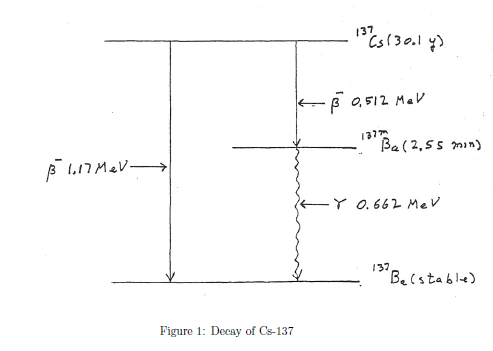
\includegraphics[scale=0.90]{apparatus.png}
\end{figure}

\section{Theory}
\indent \indent The theory section of the manual gives:

\[ N(t) = N_0e^-^\lambda ^t \] \\
\indent It's easy to derive their next statement:
\[ N(t) =  N_0e^-^\lambda ^T \]
\[ ln(\frac{N_0}{N(t)}) = \lambda T_1_/_2 \] \\
\[ T_1_/_2 = \frac{ln2}{\lambda} = \frac{0.693}{\lambda} \]
\indent Where $\frac{N_0}{N(t)} = 2 $, because $N(t)$ is half of $N_0$.

\section{Data}
\begin{figure}[H]
\centering
\hspace{-0.0in}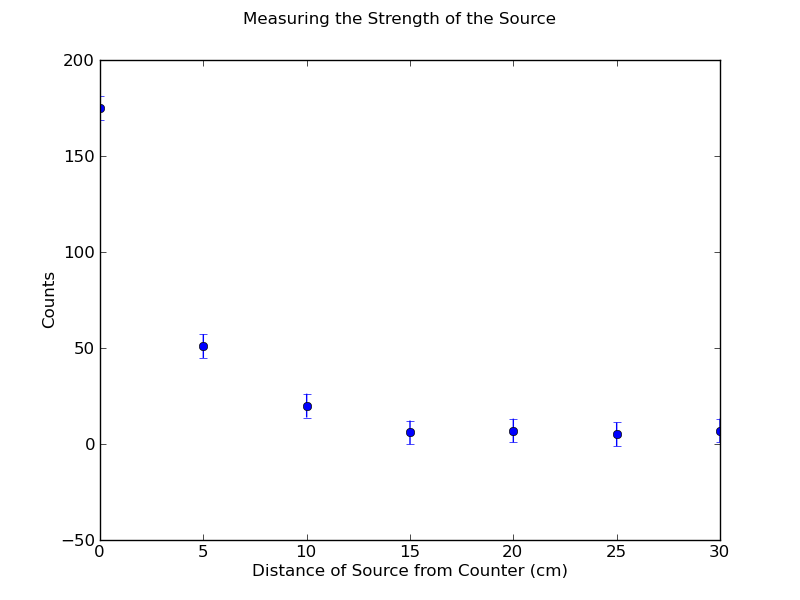
\includegraphics[scale=0.60]{Plot1.png}
\caption{Counts were recorded for .1 min each run. \label{fig:setup}}
\end{figure}

\begin{figure}[H]
\centering
\hspace{-0.0in}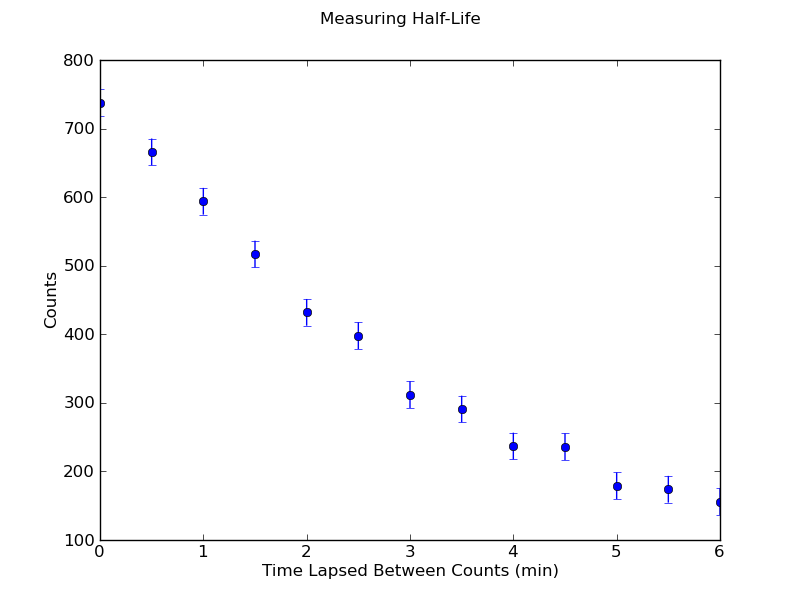
\includegraphics[scale=0.60]{Plot2.png}
\caption{Counts were recorded for .1 min each run. \label{fig:setup}}
\end{figure}

\begin{figure}[H]
\centering
\hspace{-0.0in}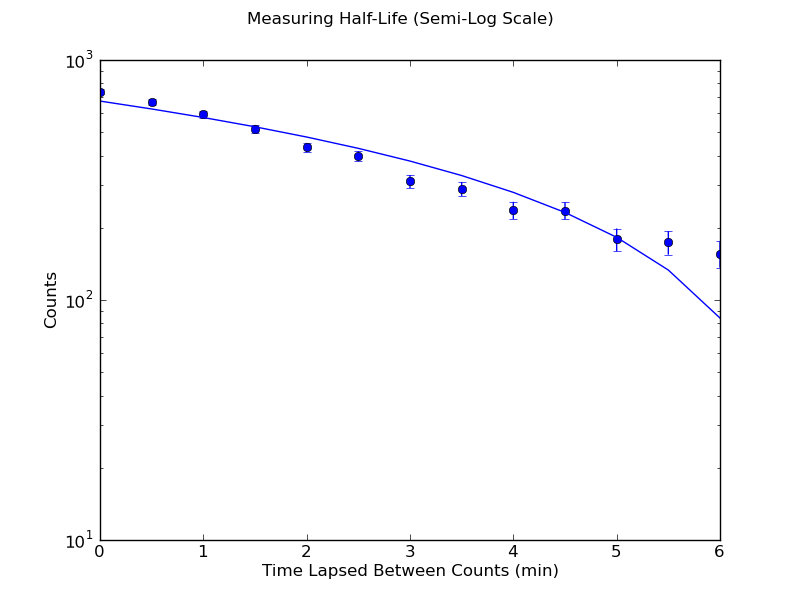
\includegraphics[scale=0.60]{Plot3.png}
\caption{Counts were recorded for .1 min each run. \label{fig:setup}}
\end{figure}

\section{Calculations}
\indent \indent Uncertainty in the Geiger Counter readings was calculated twice:
\[ \delta \sigma = \sqrt{N_a_v_g} \]
\[\delta \sigma_1 = \sqrt{38.71} = \pm 6 counts \]
\[\delta \sigma_2 = \sqrt{379.23} = \pm 19 counts \]

\indent There is also an analysis of the Half-Life data:
\[ \lambda = \frac{ln\frac{N_1}{N_2}}{t_2 - t_1} \]
\indent Using two widely spaced and convenient points:
\[ \lambda = \frac{ln\frac{594 counts}{179 counts}}{5 min - 1 min} = .3 min^-^1 \]
\indent This determines a value for $T_1_/_2$ of Barium:
\[ T_1_/_2 = \frac{.693}{.3 min^-^1} = 2.31 min \]

\section{Error Analysis}
\indent \indent There was uncertainty in readings for the distance of the source from the geiger counter in the first part of this experiment. There was uncertainty in timed readings from a stopwatch and the geiger counter. The only readings which propagated through calculations were uncertainty in counts. Finding how uncertainty propogates in a quotient:
\[\frac{\delta q}{|q|} = \sqrt{(\frac{\delta x}{x})^2 + (\frac{\delta y}{y})^2 } \]

\indent The geiger counter readings will have the same uncertainty on average:
\[\delta q = (\frac{594 counts}{179 counts})\sqrt{(\frac{19 counts}{594 counts})^2 + (\frac{19 counts}{179})^2 } = \pm .3678 \]
\indent Since this applies to the quotient of count readings, the fractional uncertainty still has some meaning. \\

\indent Percent Errors:
\[\frac{|2.55 min - 2.31 min|}{2.55 min} = 9.41 \% \]

\section{Conclusion}
\indent \indent The number I obtained is both reasonable and consistent with the accepted value. I did see what I expected to see for measuring the source strength and the half-life of metastable Barium.

\section{Questions}
\indent \indent 1. How far away does the source have to be before its presence makes no difference? \\
\indent Our data would suggest 10 cm. \\
\indent 2. How does the strength of the source fall off with distance? \\
\indent While we could have taken data at smaller intervals to make sure of this, the strength of the source appears to fall off as a negative exponential. \\
\indent 3. Source Check: Measure the strength of the Ba solution by counting for 1 min. Count the background radiation and note the time. \\
\indent There were 1257 counts after 1 minutes and we measured the backround radiation to be about 17 counts per minute. We used a new source for the second part of this lab, so 20 minutes had not passed as we were doing the source check and there was much more activity in the Barium than the manual assumed.

\end{document}